%\document{article}
\documentclass[UTF8]{ctexart}
\usepackage{listings} 
\usepackage{amsmath}
\usepackage{graphicx}
\usepackage{fancyhdr}
\usepackage{float}


\title{存储器ram}
\author{PB16030899 朱河勤}
\pagestyle{fancy}
\lhead{PB16030899 朱河勤}
\chead{存储器ram}
\rhead{2018/4/11}
\begin{document}
\maketitle
\tableofcontents

\section{实验目的}

\paragraph{1}学习如何使用ISE的IP核
\paragraph{2}学习使用Xilinx FPGA内的RAM资源
例化一个简单双端口的RAM(32bitx64)
使用coe文件对RAM进行初始化
方法


\section{实验平台}
vivado



\section{实验要求}

\subsection{功能要求}
设计一64*32bit的ram 要求
\paragraph{1}从ram中0地址和1地址读取两个数, 分别赋给reg0和reg1
\paragraph{2}利用第二次实验的结果(ALU+Regfile)进行斐波拉契运算,运算结果保存在对应的寄存器
\paragraph{3}运算结果同时保存在对应的ram地址中,即ram[0]<----->reg0, ram[1]<----->reg1,
   ram[2]<----->reg2,……

\subsection{设计要求}
\paragraph{1}实现一个顶层模块Top
\paragraph{2}实现一个control模块,完成整个运算的控制。
* 调用Ram
* 调用RegFile
* 调用ALU完成运算
* 调用control模块,完成运算控制



\section{实验分析}
\paragraph{1}设计control 模块, 用状态机进行控制
\paragraph{2}设计testbench
\paragraph{3}设计top模块,只是实例化各个模块
\section{实验结果}

\begin{figure}[H]
  \centering
  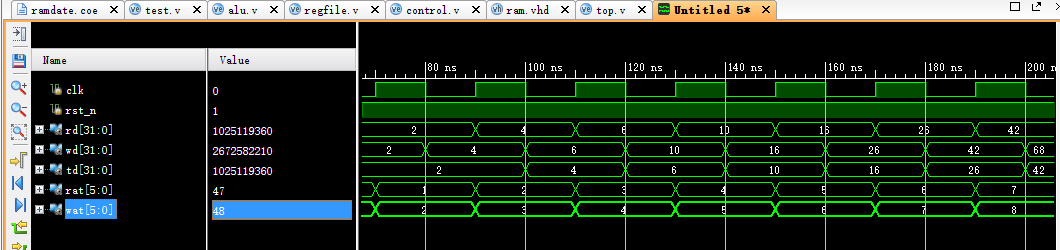
\includegraphics[width=1\textwidth]{wave.png}
\end{figure}



\section{源代码}

\begin{verbatim}
//alignmodule alu(
    input [31:0] alu_a,
    input [31:0] alu_b,
    input [4:0] alu_op,
    output reg [31:0] alu_out
    );
	always@(*)
		case (alu_op)
			0: alu_out = 0;
			1: alu_out = alu_a + alu_b;
			2: alu_out = alu_a - alu_b;
			3: alu_out = alu_a & alu_b;
			4 : alu_out = alu_a | alu_b;
			5: alu_out = alu_a ^ alu_b;
			6: alu_out = ~(alu_a | alu_b);
			default: alu_out = 0;
		endcase
endmodule

//control
module control(
	input clk,rst_n,
	//input [31:0] a,
	//input [31:0] b,
	input [31:0] aluout,
	output reg [5:0] ra=6'd0,//reg read addr
	input [31:0] rd,//reg read data
	output reg [5:0] wa=6'd0,
	output reg [31:0] wd,//reg write data
	output reg [31:0] td,//tmp data
	output reg ram_we,//reg write enable
	output reg [5:0] ram_ra,//reg read addr
	input [31:0] ram_rd//reg read data
    );
	reg [1:0] state=2'b11;//state变化3->0->1->2->2->2...
	always@(negedge clk) 
		
		if(state==2'b11) 
			begin
				ram_ra<=6'b0;
			end
		else if(state==2'b00) 
			begin
				wd<=ram_rd;
				ram_ra<=6'b1;
			end
		else if(state==2'b01)
			begin
				wd<=ram_rd;
				td<=rd; 
			end
		else if(state==2'b10) 
			begin	
				wd<=aluout;
				td<=rd; 
				ram_we=1'b1;
			end
			
	always@(posedge clk or negedge rst_n) 
		if(~rst_n)
				wa<=6'd0;
				ra<=6'd0;
				state<=2'b11;
			end
		else
			begin
				if(state==2'b11)
					begin
						state<=2'b00;
					end
				else if(state==2'b00)
					begin
						state<=2'b01;
						wa<=wa+6'd1;
					end
				else if(state==2'b01)
					begin
						ra<=ra+6'd1;
						wa<=wa+6'd1;
						state<=2'b10;
					end
				else if(state==2'b10) 
					begin
						ra<=ra+6'd1;
						wa<=wa+6'd1;
					end
				
			end
	end

endmodule
//topmodule top(
	input clk,rst_n,
	//input [31:0] a,
	//input [31:0] b,
	output  [31:0] rd,
	output  [31:0] wd,
	output [31:0] td,
	output [5:0] rat,
	output [5:0] wat
);

	wire [5:0] ra;
	wire [5:0] wa;
	
	wire [31:0] aluout;
	
	reg we=1'b1;
	
	assign rat=ra;
	assign wat=wa;
	
	wire clkb;
	wire ram_we;
	wire [5:0] ram_ra;
	wire [31:0] ram_rd;
	
	alu alu1(td,rd,5'h01,aluout);
	regfile regfile1(clk,rst_n,ra,wa,wd,we,rd);
	control control1(clk,rst_n,aluout,ra,rd,wa,wd,td,ram_we,ram_ra,ram_rd);
	ram ram1(clk,ram_we,1,wa,wd,clk,1,ram_ra,ram_rd);
	
endmodule

//regfile
module regfile(
	input	clk,
	input rst_n,
	input [5:0] rAddr1,
	input [31:0] wDin,
	output [31:0] rDout1
	integer i;
	assign rDout1=data[rAddr1];
		if(~rst_n)
		begin
			data[0]=0;
			data[1]=0;
			for(i=2; i<64; i=i+1) data[i]<=0;
		end
		else
		begin
			if(wEna)
				data[wAddr]<=wDin;
		end
endmodule

//testbench
module test(
    );
	reg clk,rst_n;
	wire [31:0] rd;
	wire [31:0] wd;
	wire [31:0] td;
	wire [5:0] rat;
	wire [5:0] wat;
 
	top test(
		.clk(clk),
		.rst_n(rst_n),
		.rd(rd),
		.wd(wd),
		.td(td),
		.rat(rat),
		.wat(wat)
	);
	  
	always #10 clk=~clk;
	initial begin
		clk=0;
		rst_n=0;
		#20;
		rst_n=1;
	end
endmodule
\end{verbatim}

\end{document}